\section{Overview}

\begin{figure}
  \centering
  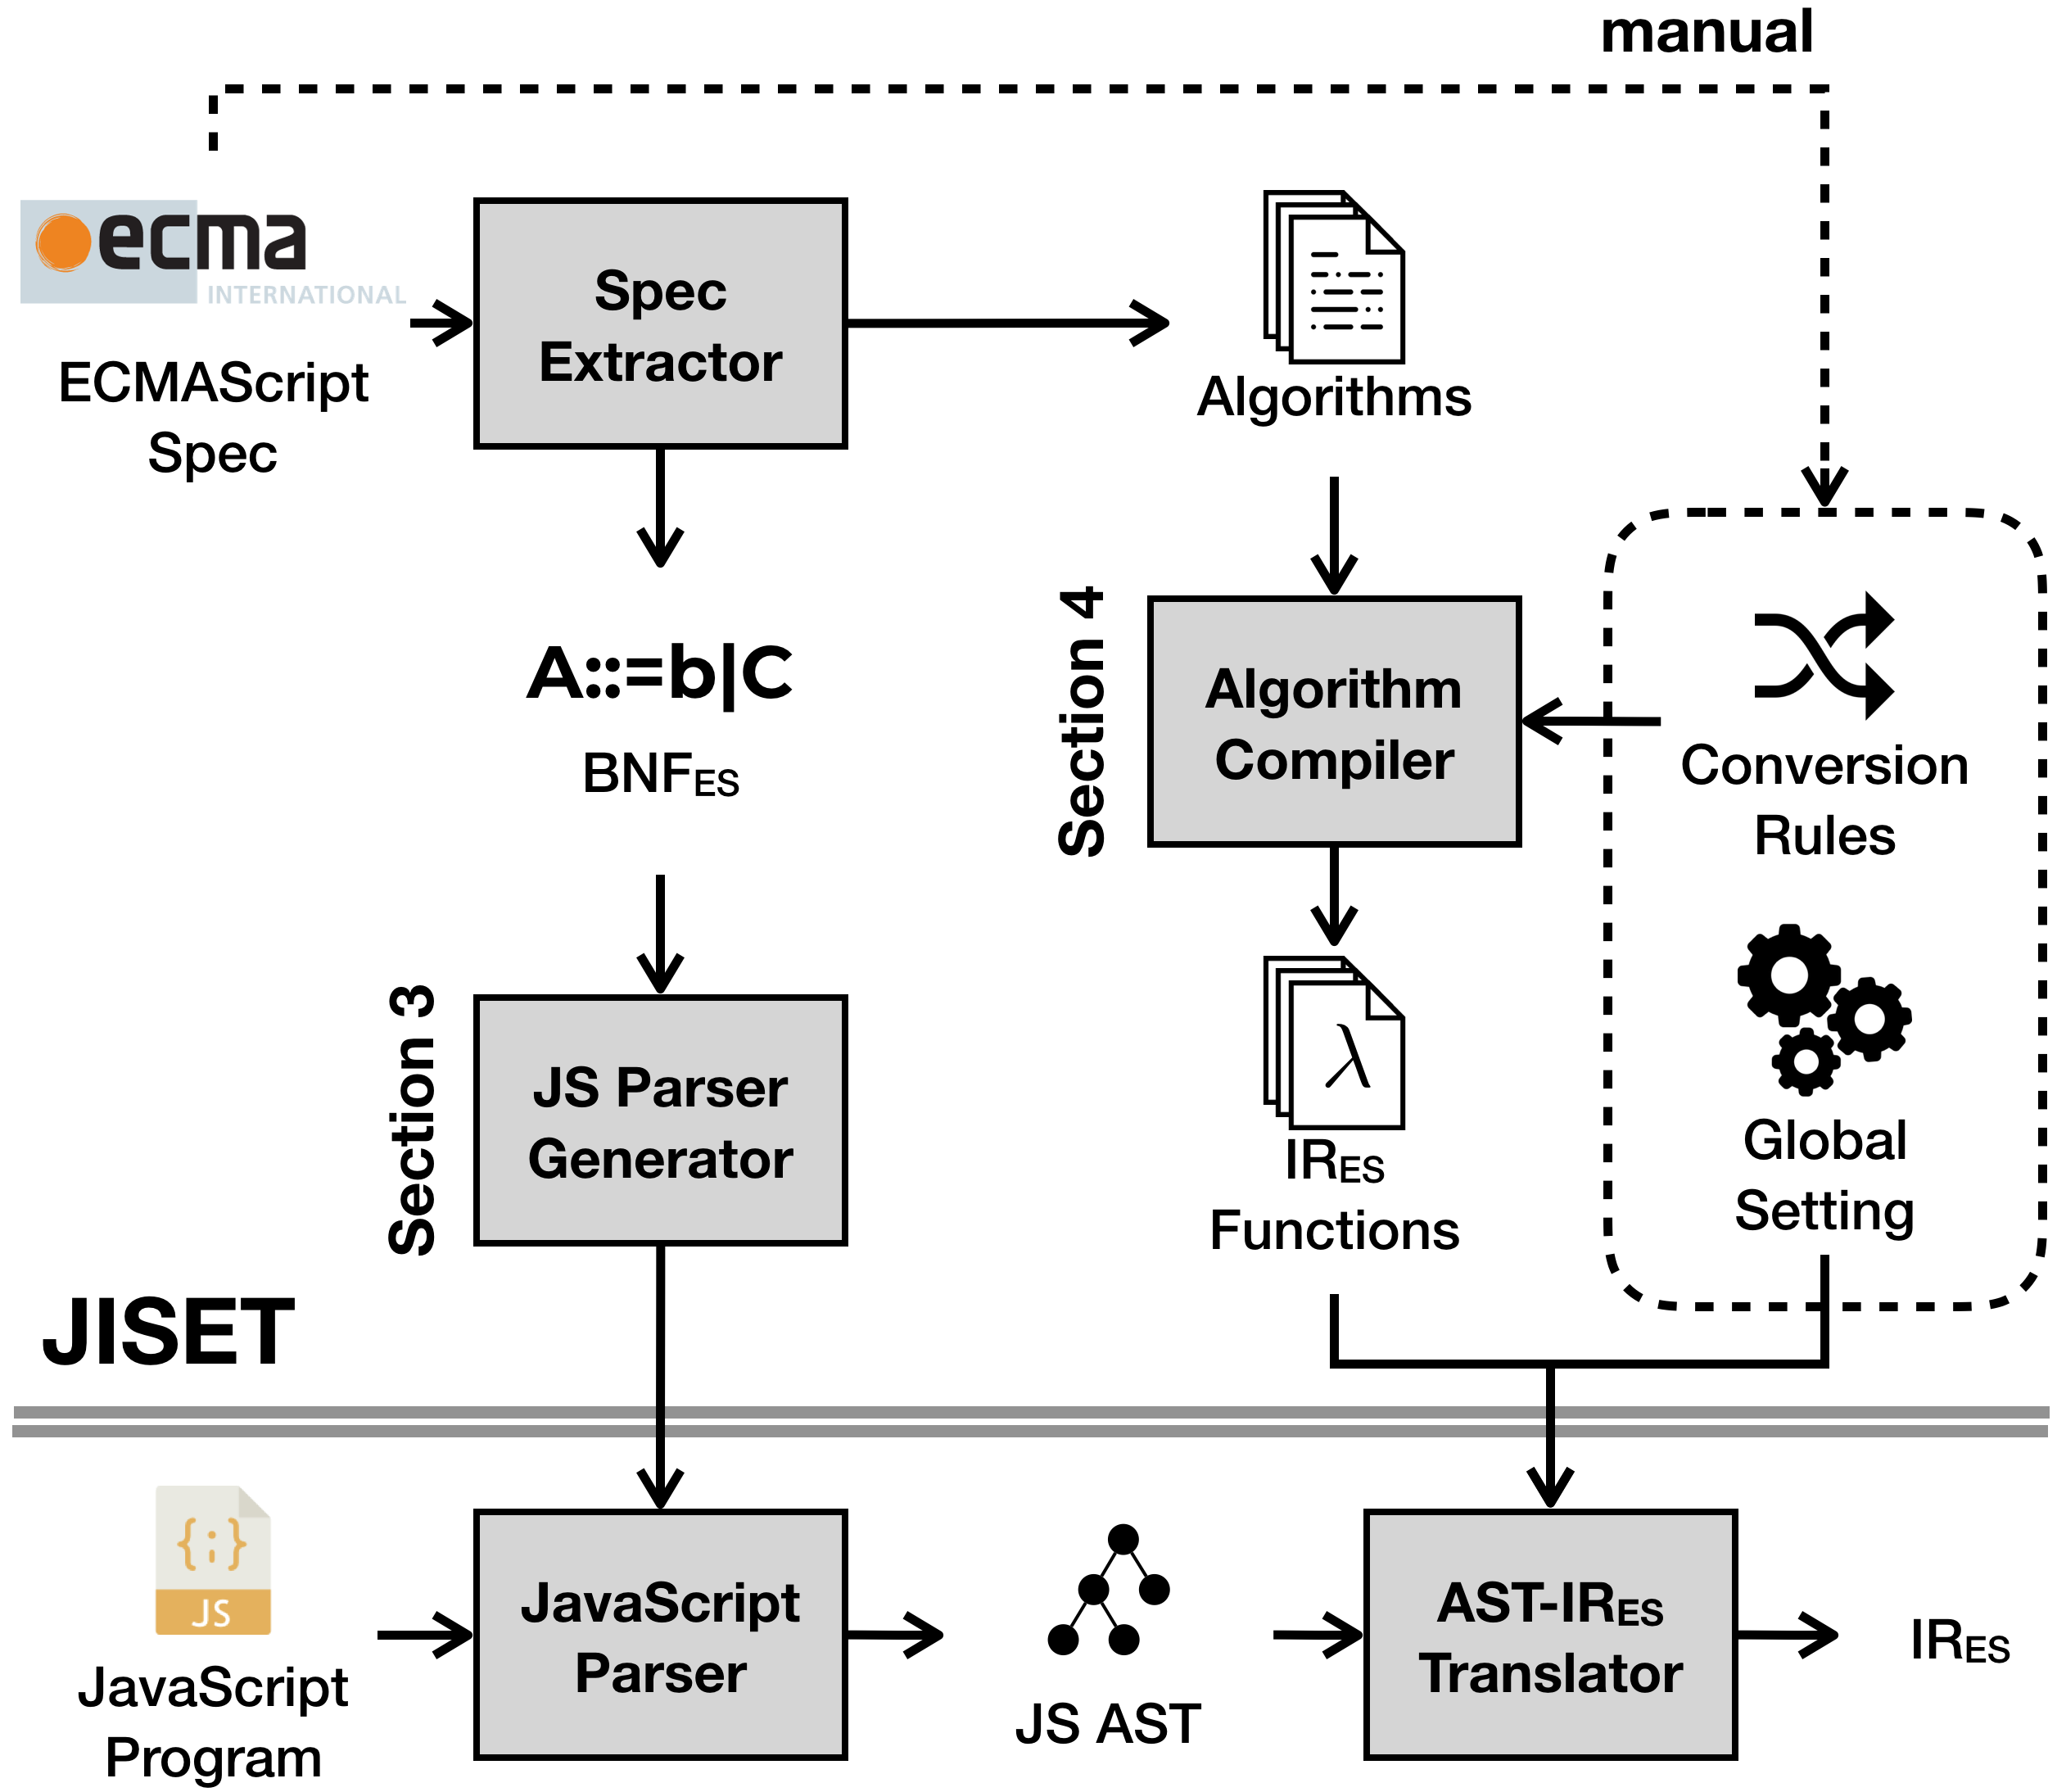
\includegraphics[width=0.5\textwidth]{img/overview.png}
  \caption{Overall structure of automatic semantics extractor (ASE)}
  \label{fig:overview}
\end{figure}

\begin{figure}
  \centering
  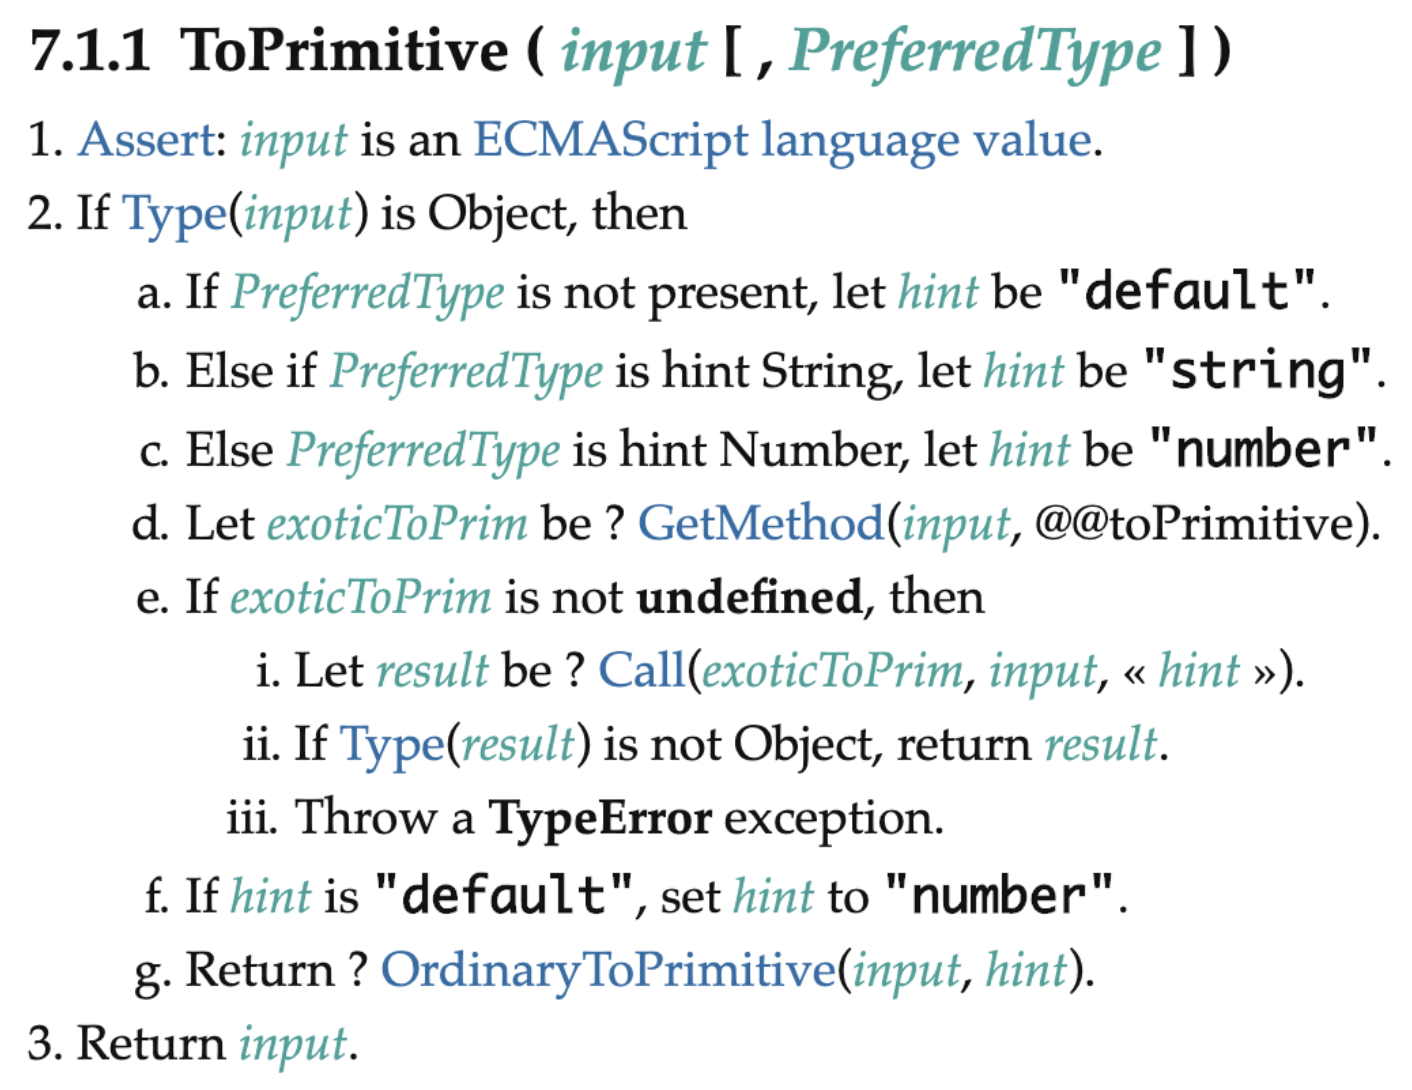
\includegraphics[height=18em]{img/to_primitive.png}
  \begin{lstlisting}[style=myCorestyle]
"ToPrimitive" (input, PreferredType) => {
  if (= (Type input) "Object") {
    if (= PreferredType absent) let hint = "default"
    else if (= PreferredType "String") let hint = "string"
    else let hint = "number"
    let exoticToPrim = ? (GetMethod input SYMBOL_toPrimitive)
    if (! (= exoticToPrim undefined)) {
      let result = ? (Call exoticToPrim input (new [hint]))
      if (! (= (Type result) "Object")) return result
      return (Throw INTRINSIC_TypeErrorPrototype)
    }
    if (= hint "default") hint = "number"
    return ? (OrdinaryToPrimitive input hint)
  }
  return input
}
  \end{lstlisting}
  \caption{\( \code{ToPrimitive} \) abstract algorithms
  and its generated core program.}
  \label{fig:to-primitive}
\end{figure}

\begin{itemize}
  \item Sytnax: automatically generate parser from ES-BNF
    \begin{itemize}
      \item ES-BNF features
      \item Packrat Parsers with 1-lookahead
      \item Example
    \end{itemize}
  \item Semantics: automatically convert abstract algorithms into Core programs
    \begin{itemize}
      \item Abstract algorithms
      \item Example
    \end{itemize}
\end{itemize}
\begin{itemize}
  \item Figure of overall structure
  \item Explanation of each module
\end{itemize}
